\documentclass{article}
\usepackage{pgfplots}
\usepackage{siunitx}
\usepackage[paperheight=2.9in,paperwidth=3.9in,margin=0in]{geometry}
\pgfplotsset{compat=1.17}
\usepgfplotslibrary{external}
\usepgfplotslibrary{fillbetween}

\tikzexternalize

\definecolor{pastelred}{rgb}{1.0, 0.41, 0.38}
\definecolor{pastelmagenta}{rgb}{0.96, 0.6, 0.76}\definecolor{pastelpink}{rgb}{1.0, 0.82, 0.86}

\begin{document}
 \pagenumbering{gobble} 
\pgfplotsset{every axis plot/.append style={line width=1pt, font=\large,}}
\tikzsetnextfilename{test.pdf}

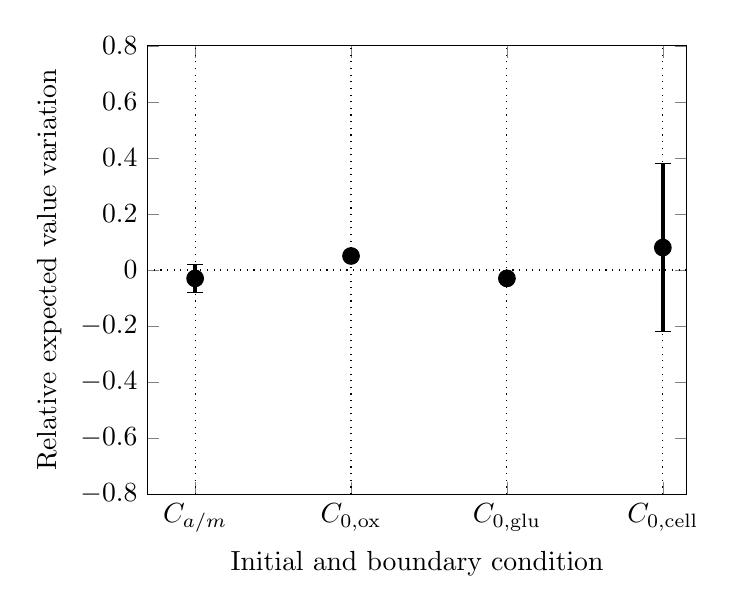
\begin{tikzpicture}
    \begin{axis}[
        ylabel = {Relative expected value variation},
        xlabel = {Initial and boundary condition},
        xmin=-0.1,
        xmax=2.15,
        xtick={0.1,0.75,1.4,2.05,2.7},
        ytick={-0.8,-0.6,-0.4,-0.2,0,0.2,0.4,0.6,0.8},
        xticklabels={$C_{a/m}$,$C_{0,\text{ox}}$,$C_{0,\text{glu}}$,$C_{0,\text{cell}}$},
        scaled y ticks = false,
        ymin=-0.8, ymax=0.8,
    ]

    \addplot[color=black,mark size=3pt, mark=*,error bars/.cd,y dir=both,y explicit, error bar style={ultra thick}] coordinates {(0.1,-0.03)+- (0,0.05)};
    \addplot[color=black,dotted] coordinates {(0.1,-0.8)(0.1,0.8)};

    \addplot[color=black, mark size=3pt, mark=*,error bars/.cd,y dir=both,y explicit] coordinates {(0.75,0.05)+- (0,0.00)};%\addlegendentry{$D_{m,\text{ox}}$}
    \addplot[color=black,dotted] coordinates {(0.75,-0.8)(0.75,0.8)};  
    
    \addplot[color=black,mark size=3pt,mark=*,error bars/.cd,y dir=both,y explicit] coordinates {(1.4,-0.03)+- (0,0.00)};%\addlegendentry{$D_{m,\text{ox}}$}
    \addplot[color=black,dotted] coordinates {(1.4,-0.8)(1.4,0.8)};  


    \addplot[color=black,mark=*,mark size=3pt, error bars/.cd,y dir=both,y explicit, error bar style={ultra thick}] coordinates {(2.05,0.08)+- (0,0.3)};%\addlegendentry{$D_{m,\text{ox}}$}
    \addplot[color=black,dotted] coordinates {(2.05,-0.8)(2.05,0.8)};  

    \addplot[color=black, dotted] coordinates {(-0.1,0)
    (2.7,0)};%\addlegendentry{$D_{m,\text{ox}}$}

    \end{axis} 
\end{tikzpicture}
\end{document}

